\documentclass[12pt]{beamer}

%\usepackage[brazil]{babel}
\usepackage[utf8]{inputenc}
\usepackage[T1]{fontenc}
\usepackage{animate}
\usepackage{amsbsy}
\usepackage{amsfonts}
\usepackage{amsmath}
\usepackage{amssymb}
\usepackage{amsthm}
\setbeamertemplate{theorems}[numbered] % to number
\usepackage[toc,page,title,titletoc]{appendix}
\usepackage{dsfont}
\usepackage{esvect}
\usepackage[labelfont=bf]{caption}
%\usepackage{subcaption}
\usepackage{float}
\usepackage[Glenn]{fncychap}%Sonny %Conny %Lenny %Glenn %Renje %Bjarne %Bjornstrup
\usepackage{graphicx}
\usepackage{subfig}
\usepackage{indentfirst}%Para indentar os paragrafos automáticamente
\usepackage{lipsum}
\usepackage{longtable}
\usepackage{mathtools}
\usepackage{listings}%Inserir codigo do R no latex
\usepackage{multirow}
\usepackage{multicol}
\usepackage{csquotes}
\usepackage[maxcitenames=2,terseinits=true,natbib=true, style=authoryear, maxbibnames=99]{biblatex}
\addbibresource{../Referencias/Referencias.bib}
\usepackage[figuresright]{rotating}
\usepackage{spalign}
\usepackage{pgfplots}
\pgfplotsset{compat=1.17}
\usepackage{tikz}
\usepackage{fontawesome}
\usepackage{color, colortbl}
\usepackage{url}
\usepackage{cancel}
\usepackage{accents}
\usepackage{bm}
\usepackage{ragged2e}%para justificar o texto dentro de algum ambiente
\definecolor{Gray}{gray}{0.9}
\definecolor{LightCyan}{rgb}{0.88,1,1}


\usepackage[all]{xy}
\usepackage{hyperref,bookmark}
\hypersetup{
  colorlinks=true,
  linkcolor=blue,
  citecolor=red,
  filecolor=blue,
  urlcolor=blue,
}

\usetheme{Madrid}
\usecolortheme[RGB={193,0,0}]{structure}

%\setbeamertemplate{footline}[frame number]
%\setbeamertemplate{footline}[text line]{%
%  \parbox{\linewidth}{\vspace*{-8pt}\hfill\date{}\hfill\insertshortauthor\hfill\insertpagenumber}}
\beamertemplatenavigationsymbolsempty
\renewcommand{\vec}[1]{\mbox{\boldmath$#1$}}
\newtheorem{Teorema}{Teorema}
\newtheorem{Proposicao}{Proposição}
\newtheorem{definicao}{Definição}
\newtheorem{Corolario}{Corolário}
\newtheorem{Demonstracao}{Demonstração}
\newcommand{\bx}{\ensuremath{\bar{x}}}
\newcommand{\Ho}{\ensuremath{H_{0}}}
\newcommand{\Hi}{\ensuremath{H_{1}}}
\newcommand{\at}[2][]{#1|_{#2}}
\newcommand\xuparrow[1][2ex]{%
   \mathrel{\rotatebox{-90}{$\xleftarrow{\rule{#1}{0pt}}$}}
}
\apptocmd{\frame}{}{\justifying}{} % Allow optional arguments after frame.

\makeatletter
\setbeamertemplate{footline}
{
  \leavevmode%
  \hbox{%
  \begin{beamercolorbox}[wd=.3\paperwidth,ht=2.25ex,dp=1ex,center]{author in head/foot}%
    \usebeamerfont{author in head/foot}\mytext
  \end{beamercolorbox}%
  \begin{beamercolorbox}[wd=.3\paperwidth,ht=2.25ex,dp=1ex,center]{title in head/foot}%
    \usebeamerfont{title in head/foot}\mytextt
  \end{beamercolorbox}%
  \begin{beamercolorbox}[wd=.35\paperwidth,ht=2.25ex,dp=1ex,right]{site in head/foot}%
    \usebeamerfont{site in head/foot}\mytexttt\hspace*{2em}
    \insertframenumber{} / \inserttotalframenumber\hspace*{2ex} 
  \end{beamercolorbox}}%
  \vskip0pt%
}
\makeatother

\providecommand{\arcsin}{} \renewcommand{\arcsin}{\hspace{2pt}\textrm{arcsen}}
\providecommand{\sin}{} \renewcommand{\sin}{\hspace{2pt}\textrm{sen}}
\newcommand{\N}{\rm I\!N}
\newcommand{\I}{\rm I\!I}
\newcommand{\R}{\rm I\!R}
\newcommand{\Sim}{\overset{\text{iid}}{\sim}}
\newcommand{\Lim}{{\displaystyle \lim_{n\to\infty}}}
\newcommand{\LimInf}{{\displaystyle \liminf_{n\to\infty}}}
\newcommand{\rightLim}{\xrightarrow[n\rightarrow\infty]{}}
\newcommand{\Sumi}{{\displaystyle \sum_{i=1}^{n}}}
\newcommand{\Int}{{\displaystyle \int_{-\infty}^{+\infty}}}
\newcommand{\ConvD}{\overset{D}{\rightarrow}}
\newcommand{\ConvP}{\overset{P}{\rightarrow}}
\newcommand{\Prodi}{{\displaystyle \prod_{i=1}^{n}}}
\newcommand{\SetaUP}[2]{\underset{\mathclap{\substack{\xuparrow[30pt] \\ #1}}}{#2}}
%\newcommand{\SetaInclinada}[2]{\underset{\mathclap{\substack{\rotatebox{135}{\xuparrow[30pt] \\ #1}}}}{#2}}
\newcommand{\Home}{\begin{tikzpicture}
\node[scale=2] at (3,4) {\text{Para}~\faHome};
\end{tikzpicture}}
\newcommand{\vecX}{\boldsymbol{X}}
\newcommand{\Implica}[1]{\xRightarrow{#1}}
\newcommand{\SeSe}{\iff}
\newcommand{\EscoreA}{\dfrac{\partial}{\partial\theta}\log{f(x,\theta)}}
\newcommand{\EscoreB}{\dfrac{\partial^{2}}{\partial\theta^{2}}\log{f(x,\theta)}}
\newcommand{\cqd}{\text{cqd}~\blacksquare}
\newcommand{\seqX}{$X_{1},\ldots,X_{n}$}
\newcommand{\seqY}{$Y_{1},\ldots,Y_{n}$}
\newcommand{\tend}[1]{\hbox{\oalign{$\bm{#1}$\crcr\hidewidth$\scriptscriptstyle\bm{\sim}$\hidewidth}}}

%\newtheorem{Teorema}{Teorema}
%\newtheorem{Proposicao}{Proposição}
%\newtheorem{Definicao}{Definição}
%\newtheorem{Corolario}{Corolário}
%\newtheorem{Demonstracao}{Demonstração}

\titlegraphic{\hspace*{8cm}\href{https://fsbmat-ufv.github.io/}{
\includegraphics[width=2cm]{figs/mylogo.png}}
}

%Continuar a numeracao em slides diferentes
\newcounter{saveenumi}
\newcommand{\seti}{\setcounter{saveenumi}{\value{enumi}}}
\newcommand{\conti}{\setcounter{enumi}{\value{saveenumi}}}

\resetcounteronoverlays{saveenumi}

% Layout da pagina
\hypersetup{pdfpagelayout=SinglePage}

%Para o \pause funcionar dentro do ambiente align
\makeatletter
\let\save@measuring@true\measuring@true
\def\measuring@true{%
  \save@measuring@true
  \def\beamer@sortzero##1{\beamer@ifnextcharospec{\beamer@sortzeroread{##1}}{}}%
  \def\beamer@sortzeroread##1<##2>{}%
  \def\beamer@finalnospec{}%
}
\makeatother
\usepackage[brazil]{babel}
\usepackage[utf8]{inputenc}
\usepackage[T1]{fontenc}
\usepackage{animate}
\usepackage{amsbsy}
\usepackage{amsfonts}
\usepackage{amsmath}
\usepackage{amssymb}
\usepackage{amsthm}
\setbeamertemplate{theorems}[numbered] % to number
\usepackage[toc,page,title,titletoc]{appendix}
\usepackage{dsfont}
\usepackage{esvect}
\usepackage[labelfont=bf]{caption}
%\usepackage{subcaption}
\usepackage{float}
\usepackage[Glenn]{fncychap}%Sonny %Conny %Lenny %Glenn %Renje %Bjarne %Bjornstrup
\usepackage{graphicx}
\usepackage{subfig}
\usepackage{indentfirst}%Para indentar os paragrafos automáticamente
\usepackage{lipsum}
\usepackage{longtable}
\usepackage{mathtools}
\usepackage{listings}%Inserir codigo do R no latex
\usepackage{multirow}
\usepackage{multicol}
\usepackage{csquotes}
\usepackage[maxcitenames=2,terseinits=true,natbib=true, style=authoryear, maxbibnames=99]{biblatex}
\addbibresource{../Referencias/Referencias.bib}
\usepackage[figuresright]{rotating}
\usepackage{spalign}
\usepackage{pgfplots}
\pgfplotsset{compat=1.17}
\usepackage{tikz}
\usepackage{fontawesome}
\usepackage{color, colortbl}
\usepackage{url}
\usepackage{cancel}
\usepackage{accents}
\usepackage{bm}
\usepackage{ragged2e}%para justificar o texto dentro de algum ambiente
\definecolor{Gray}{gray}{0.9}
\definecolor{LightCyan}{rgb}{0.88,1,1}


\usepackage[all]{xy}
\usepackage{hyperref,bookmark}
\hypersetup{
  colorlinks=true,
  linkcolor=blue,
  citecolor=red,
  filecolor=blue,
  urlcolor=blue,
}

\usetheme{Madrid}
\usecolortheme[RGB={193,0,0}]{structure}

%\setbeamertemplate{footline}[frame number]
%\setbeamertemplate{footline}[text line]{%
%  \parbox{\linewidth}{\vspace*{-8pt}\hfill\date{}\hfill\insertshortauthor\hfill\insertpagenumber}}
\beamertemplatenavigationsymbolsempty
\renewcommand{\vec}[1]{\mbox{\boldmath$#1$}}
\newtheorem{Teorema}{Teorema}
\newtheorem{Proposicao}{Proposição}
\newtheorem{definicao}{Definição}
\newtheorem{Corolario}{Corolário}
\newtheorem{Demonstracao}{Demonstração}
\newcommand{\bx}{\ensuremath{\bar{x}}}
\newcommand{\Ho}{\ensuremath{H_{0}}}
\newcommand{\Hi}{\ensuremath{H_{1}}}
\newcommand{\at}[2][]{#1|_{#2}}
\newcommand\xuparrow[1][2ex]{%
   \mathrel{\rotatebox{-90}{$\xleftarrow{\rule{#1}{0pt}}$}}
}
\apptocmd{\frame}{}{\justifying}{} % Allow optional arguments after frame.

\makeatletter
\setbeamertemplate{footline}
{
  \leavevmode%
  \hbox{%
  \begin{beamercolorbox}[wd=.3\paperwidth,ht=2.25ex,dp=1ex,center]{author in head/foot}%
    \usebeamerfont{author in head/foot}\mytext
  \end{beamercolorbox}%
  \begin{beamercolorbox}[wd=.3\paperwidth,ht=2.25ex,dp=1ex,center]{title in head/foot}%
    \usebeamerfont{title in head/foot}\mytextt
  \end{beamercolorbox}%
  \begin{beamercolorbox}[wd=.35\paperwidth,ht=2.25ex,dp=1ex,right]{site in head/foot}%
    \usebeamerfont{site in head/foot}\mytexttt\hspace*{2em}
    \insertframenumber{} / \inserttotalframenumber\hspace*{2ex} 
  \end{beamercolorbox}}%
  \vskip0pt%
}
\makeatother

\providecommand{\arcsin}{} \renewcommand{\arcsin}{\hspace{2pt}\textrm{arcsen}}
\providecommand{\sin}{} \renewcommand{\sin}{\hspace{2pt}\textrm{sen}}
\newcommand{\N}{\rm I\!N}
\newcommand{\I}{\rm I\!I}
\newcommand{\R}{\rm I\!R}
\newcommand{\Sim}{\overset{\text{iid}}{\sim}}
\newcommand{\Lim}{{\displaystyle \lim_{n\to\infty}}}
\newcommand{\LimInf}{{\displaystyle \liminf_{n\to\infty}}}
\newcommand{\rightLim}{\xrightarrow[n\rightarrow\infty]{}}
\newcommand{\Sumi}{{\displaystyle \sum_{i=1}^{n}}}
\newcommand{\Int}{{\displaystyle \int_{-\infty}^{+\infty}}}
\newcommand{\ConvD}{\overset{D}{\rightarrow}}
\newcommand{\ConvP}{\overset{P}{\rightarrow}}
\newcommand{\Prodi}{{\displaystyle \prod_{i=1}^{n}}}
\newcommand{\SetaUP}[2]{\underset{\mathclap{\substack{\xuparrow[30pt] \\ #1}}}{#2}}
%\newcommand{\SetaInclinada}[2]{\underset{\mathclap{\substack{\rotatebox{135}{\xuparrow[30pt] \\ #1}}}}{#2}}
\newcommand{\Home}{\begin{tikzpicture}
\node[scale=2] at (3,4) {\text{Para}~\faHome};
\end{tikzpicture}}
\newcommand{\vecX}{\boldsymbol{X}}
\newcommand{\Implica}[1]{\xRightarrow{#1}}
\newcommand{\SeSe}{\iff}
\newcommand{\EscoreA}{\dfrac{\partial}{\partial\theta}\log{f(x,\theta)}}
\newcommand{\EscoreB}{\dfrac{\partial^{2}}{\partial\theta^{2}}\log{f(x,\theta)}}
\newcommand{\cqd}{\text{cqd}~\blacksquare}
\newcommand{\seqX}{$X_{1},\ldots,X_{n}$}
\newcommand{\seqY}{$Y_{1},\ldots,Y_{n}$}
\newcommand{\tend}[1]{\hbox{\oalign{$\bm{#1}$\crcr\hidewidth$\scriptscriptstyle\bm{\sim}$\hidewidth}}}

%\newtheorem{Teorema}{Teorema}
%\newtheorem{Proposicao}{Proposição}
%\newtheorem{Definicao}{Definição}
%\newtheorem{Corolario}{Corolário}
%\newtheorem{Demonstracao}{Demonstração}

\titlegraphic{\hspace*{8cm}\href{https://fsbmat-ufv.github.io/}{
\includegraphics[width=2cm]{figs/mylogo.png}}
}

%Continuar a numeracao em slides diferentes
\newcounter{saveenumi}
\newcommand{\seti}{\setcounter{saveenumi}{\value{enumi}}}
\newcommand{\conti}{\setcounter{enumi}{\value{saveenumi}}}

\resetcounteronoverlays{saveenumi}

% Layout da pagina
\hypersetup{pdfpagelayout=SinglePage}

%Para o \pause funcionar dentro do ambiente align
\makeatletter
\let\save@measuring@true\measuring@true
\def\measuring@true{%
  \save@measuring@true
  \def\beamer@sortzero##1{\beamer@ifnextcharospec{\beamer@sortzeroread{##1}}{}}%
  \def\beamer@sortzeroread##1<##2>{}%
  \def\beamer@finalnospec{}%
}
\makeatother

\title{Inferência Estatística II}
\author{Prof. Fernando de Souza Bastos\texorpdfstring{\\ fernando.bastos@ufv.br}{}}
\institute{Departamento de Estatística\texorpdfstring{\\ Programa de Pós-Graduação em Estatística Aplicada e Biometria}\texorpdfstring{\\ Universidade Federal de Viçosa}{}\texorpdfstring{\\ Campus UFV - Viçosa}{}}
\date{}
\newcommand\mytext{Aula 1}
\newcommand\mytextt{Fernando de Souza Bastos}
\newcommand\mytexttt{\url{https://est711.github.io/}}


\begin{document}
%\SweaveOpts{concordance=TRUE}

\frame{\titlepage}

\begin{frame}{}
\frametitle{\bf Sumário}
\tableofcontents
\end{frame}

\section{Preliminares}
\begin{frame}{}
\frametitle{}
\begin{block}{}
\justifying
A Inferência Estatística é um ramo da Estatística que se dedica a tirar conclusões sobre uma população com base em uma amostra representativa dessa população. Surgida no início do século XX, essa área se desenvolveu como uma resposta à necessidade de generalizar os resultados obtidos a partir de dados amostrais, permitindo a extrapolação de informações de forma rigorosa e fundamentada.
\end{block}
\end{frame}

\begin{frame}{}
\begin{block}{}
\justifying
Dentre os principais pesquisadores, destacam-se Ronald Fisher, Jerzy Neyman e Egon Pearson, que foram responsáveis por desenvolver a Teoria da Estimação e a Teoria dos Testes de Hipóteses. Além desses, outros autores importantes incluem William Gosset (conhecido como Student), que criou o teste t de Student, e Harold Hotelling, que desenvolveu a Teoria da Distribuição Multivariada.
\end{block}\pause
\begin{block}{Sugestão de Leitura:}
\justifying
Uma Senhora Toma Chá...: Como a Estatística Revolucionou a Ciência no Século XX.\cite{salsburg}
\end{block}
\end{frame}

\begin{frame}{}
	\begin{block}{}
		\begin{columns}%[T] % O argumento [T] alinha as colunas pelo topo
			
			\begin{column}{0.5\textwidth} % Largura da coluna de texto
				\vfill
				\centering
				\justifying
				Ronald A. Fisher (1890-1962) estatístico e geneticista britânico, desenvolveu a análise de variância (ANOVA) e o teste de significância, e foi um pioneiro no uso de experimentos controlados para validar hipóteses científicas.
			\end{column}
			
			\begin{column}{0.5\textwidth} % Largura da coluna da figura
				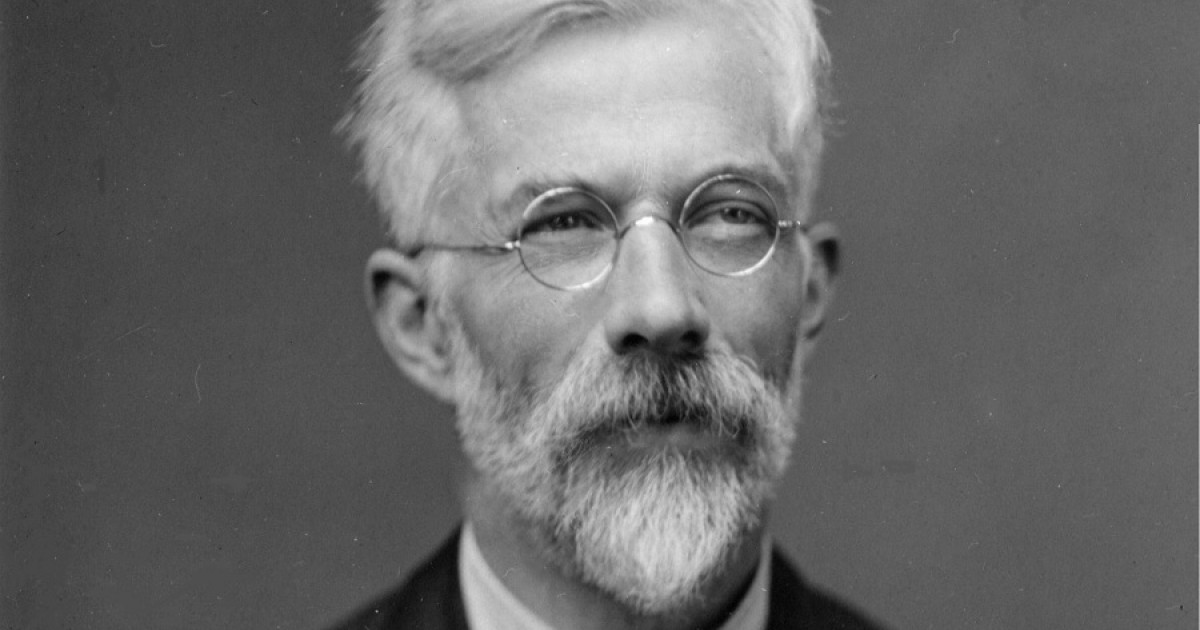
\includegraphics[width=\textwidth]{figs/Fisher.jpg} % Substitua 'imagem.png' pelo nome do seu arquivo de imagem
			\end{column}
			
		\end{columns}
	\end{block}
\end{frame}

\begin{frame}{}
	\begin{block}{}
		\begin{columns} % O argumento [T] alinha as colunas pelo topo
			
			\begin{column}{0.6\textwidth} % Largura da coluna de texto
				\vfill
				\centering
				\justifying
				Karl Pearson (1857-1936) foi um estatístico e biométrico britânico, conhecido por desenvolver o conceito de correlação e regressão, além de fundar o campo da biometria. Ele também fez importantes contribuições para a teoria da probabilidade e a inferência estatística.
			\end{column}
			
			\begin{column}{0.3\textwidth} % Largura da coluna da figura
				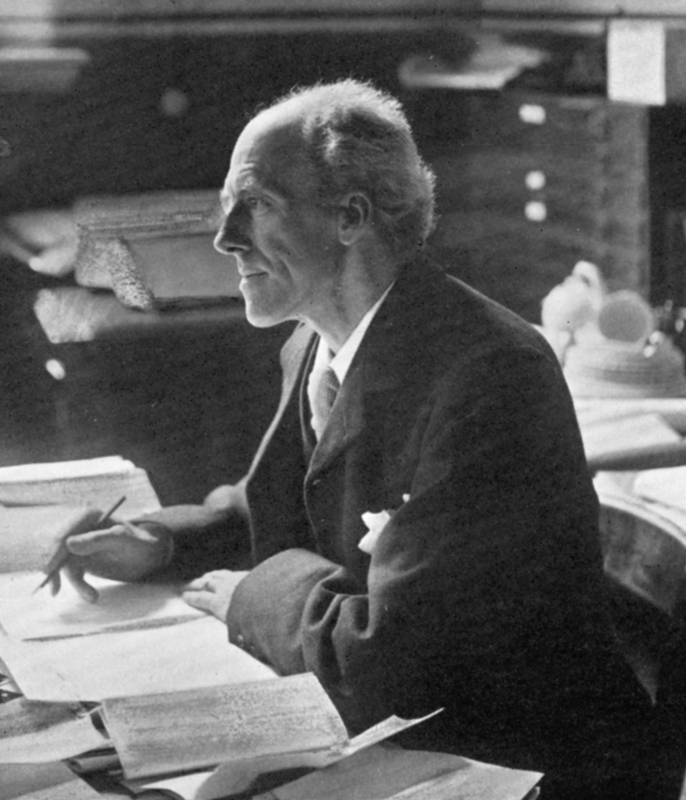
\includegraphics[width=0.7\textwidth]{figs/KarlPearson.jpg} % Substitua 'imagem.png' pelo nome do seu arquivo de imagem
			\end{column}
			
		\end{columns}
	\end{block}
\end{frame}

\begin{frame}{}
	\begin{block}{}
		\begin{columns} % O argumento [T] alinha as colunas pelo topo
			
			\begin{column}{0.6\textwidth} % Largura da coluna de texto
				\vfill
				\centering
				\justifying
				Egon Pearson (1895-1980) foi um estatístico britânico e filho de Karl Pearson. Ele é mais conhecido por suas contribuições à teoria estatística, especialmente no desenvolvimento da teoria dos testes de hipóteses. Juntamente com Ronald A. Fisher, ele desenvolveu o conceito de erro tipo I e erro tipo II em testes de hipóteses. 
			\end{column}
			
			\begin{column}{0.3\textwidth} % Largura da coluna da figura
				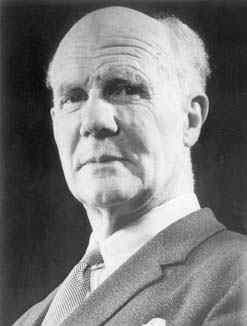
\includegraphics[width=0.7\textwidth]{figs/Pearson.jpeg} % Substitua 'imagem.png' pelo nome do seu arquivo de imagem
			\end{column}
			
		\end{columns}
	\end{block}
\end{frame}

\begin{frame}{}
	\begin{block}{}
		\begin{columns} % O argumento [T] alinha as colunas pelo topo
			
			\begin{column}{0.6\textwidth} % Largura da coluna de texto
				\vfill
				\centering
				\justifying
				Jerzy Neyman (1894-1981) polonês de renome internacional, conhecido por suas contribuições fundamentais à teoria estatística. Neyman é famoso pelo desenvolvimento do método de intervalos de confiança e pelo conceito de testes de hipóteses que incluem o teste de significância.Também desempenhou um papel crucial na fundação do campo da estatística matemática e na educação estatística.
			\end{column}
			
			\begin{column}{0.3\textwidth} % Largura da coluna da figura
				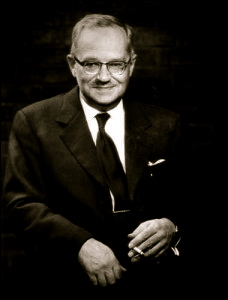
\includegraphics[width=0.7\textwidth]{figs/Neyman.jpg} % Substitua 'imagem.png' pelo nome do seu arquivo de imagem
			\end{column}
			
		\end{columns}
	\end{block}
\end{frame}

\begin{frame}{}
	\begin{block}{}
		\begin{columns} % O argumento [T] alinha as colunas pelo topo
			
			\begin{column}{0.6\textwidth} % Largura da coluna de texto
				\vfill
				\centering
				\justifying
				William Sealy Gosset (1876-1937) foi um estatístico britânico que trabalhou sob o pseudônimo "Student". Gosset desenvolveu o teste t enquanto trabalhava para a cervejaria Guinness, onde lidava com amostras pequenas e necessitava de métodos estatísticos apropriados para análise de dados limitados.
			\end{column}
			
			\begin{column}{0.3\textwidth} % Largura da coluna da figura
				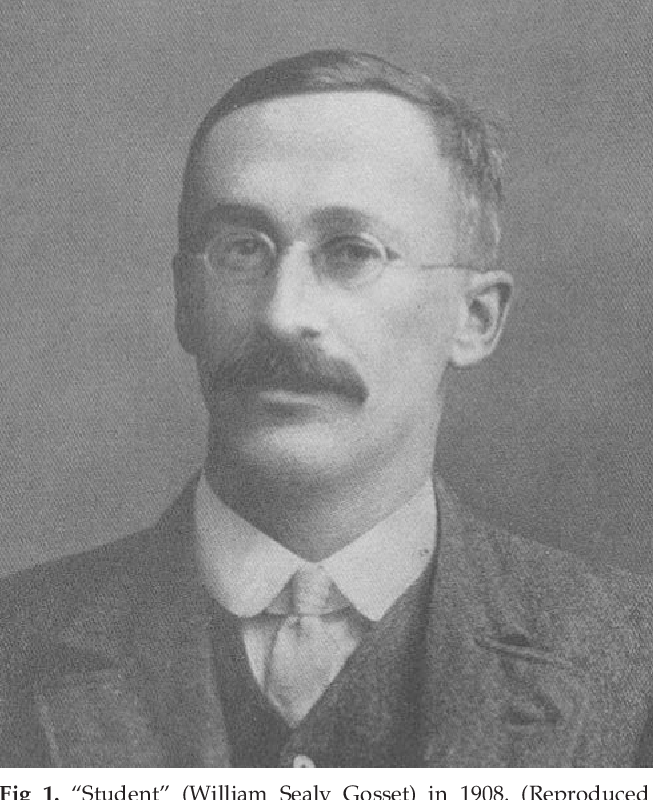
\includegraphics[width=0.7\textwidth]{figs/Gosset.png} % Substitua 'imagem.png' pelo nome do seu arquivo de imagem
			\end{column}
			
		\end{columns}
	\end{block}
\end{frame}

\begin{frame}{}
	\begin{block}{}
		\begin{columns} % O argumento [T] alinha as colunas pelo topo
			
			\begin{column}{0.6\textwidth} % Largura da coluna de texto
				\vfill
				\centering
				\justifying
				Harold Hotelling (1895-1973) foi um estatístico e economista americano, conhecido por suas contribuições significativas à estatística multivariada e à econometria. Entre suas realizações notáveis estão o desenvolvimento do teste de Hotelling, que é uma generalização do teste t para múltiplas variáveis. Suas ideias e métodos continuam a influenciar áreas como Análise Estatística, Economia e Ciência de dados.
			\end{column}
			
			\begin{column}{0.3\textwidth} % Largura da coluna da figura
				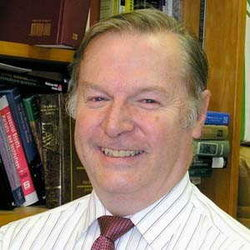
\includegraphics[width=0.7\textwidth]{figs/Hotelling.jpg} % Substitua 'imagem.png' pelo nome do seu arquivo de imagem
			\end{column}
			
		\end{columns}
	\end{block}
\end{frame}

%\begin{frame}{}
%    \begin{block}{}
%        \justifying
%        \nocite{hogg, casella2021statistical}
%        A Estatística é uma disciplina rica e diversificada, com uma longa história de contribuição de diversos pesquisadores notáveis. Além dos nomes frequentemente mencionados, muitos outros cientistas também desempenharam papéis cruciais no desenvolvimento da área. Cada um trouxe inovações e técnicas que ampliaram a capacidade da Estatística para interpretar dados e fazer previsões precisas.
%    \end{block}
%\end{frame}
%
%\begin{frame}{}
%	\begin{block}{}
%		\justifying
%		O estudo aprofundado da inferência estatística é particularmente importante, pois é a base para muitas das técnicas utilizadas na análise de dados e na tomada de decisões informadas. A inferência estatística nos permite tirar conclusões sobre uma população com base em uma amostra, calcular intervalos de confiança e realizar testes de hipóteses para validar teorias. 
%	\end{block}
%\pause
%	\begin{block}{}
%		\justifying
%		Compreender esses métodos é essencial para aplicar a Estatística de maneira eficaz em diversos campos, desde a pesquisa científica até a análise de mercado e além. Portanto, um conhecimento sólido de inferência estatística é fundamental para qualquer profissional que deseje utilizar dados para gerar insights valiosos e tomar decisões fundamentadas.
%	\end{block}
%\end{frame}

%\begin{frame}{}
%    \begin{block}{Um curso completo de Inferência Estatística deve conter:}
%        \justifying
%        \begin{enumerate}
%            \item Teoria da Probabilidade: fundamentos da teoria da probabilidade, definição de variáveis aleatórias e distribuições de probabilidade. (EST 610 e EST 710)
%
%            \item Estatística Descritiva: cálculo de medidas de tendência central e dispersão, construção de gráficos e tabelas descritivas.  (EST 105, EST 106 e EST 611)
%
%            \item Amostragem: métodos de amostragem, definição de amostra representativa e não representativa. (EST 627 - Amostragem e Testes Não Paramétricos)
%
%            \item Teoria da Estimação: intervalos de confiança, estimativas pontuais, métodos de estimação. (EST 611 e EST 711)
%
%            \item Testes de Hipóteses: definição de hipóteses nulas e alternativas, tipos de erros, níveis de significância, testes de significância. (EST 711)
%            \seti
%\end{enumerate}
%    \end{block}
%\end{frame}
%
%\begin{frame}{}
%    \begin{block}{Um curso completo de Inferência Estatística deve conter:}
%        \justifying
%        \begin{enumerate}
%        \conti
%             \item Regressão Linear: definição e aplicação da regressão linear simples e múltipla, análise de variância, interpretação de resultados.(EST 744)
%
%            \item Análise de Variância (ANOVA): definição e aplicação da ANOVA de um e dois fatores, análise de componentes principais. (EST 622, EST 630, EST 631, EST 711 e EST 722)
%
%            \item Métodos Não Paramétricos: testes de hipóteses não paramétricos, análise de dados categóricos. (EST 627)
%
%            \item Inferência Bayesiana: fundamentos da teoria bayesiana, cálculo de probabilidades a posteriori, interpretação de resultados. (EST 613)
%            \seti
%        \end{enumerate}
%    \end{block}
%\end{frame}
%
%\begin{frame}{}
%    \begin{block}{Um curso completo de Inferência Estatística deve conter:}
%        \justifying
%        \begin{enumerate}
%        \conti
%             \item Métodos Computacionais em Inferência Estatística: uso de software estatístico, programação em linguagem R, simulação de dados. (EST 629)
%        \end{enumerate}
%    \end{block}
%    \pause 
%    \begin{block}{}
%    \justifying
%        Esses conteúdos são fundamentais para o domínio da Inferência Estatística e podem ser adaptados de acordo com o nível de conhecimento e aplicação desejados pelo curso. Sugiro aprender também, programação, python e \LaTeX.
%    \end{block}    
%\end{frame}

\section{Revisão Sobre Estimação Pontual}

\begin{frame}{Revisão de Estimação Pontual}
	\begin{block}{}
		\justifying
		\nocite{hogg, casella2021statistical}
		Em um problema Estatístico típico, temos uma variável aleatória $X$ de interesse, mas sua função de densidade de probabilidade $f(x)$ ou sua função de massa de probabilidade $p(x)$ não é conhecida. Nossa ignorância pode ser classificada de maneira geral de duas formas:
	\end{block}
	\pause
	\begin{block}{Classificações da Ignorância}
		\begin{enumerate}
			\item $f(x)$ ou $p(x)$ é completamente desconhecida.
			\item A forma de $f(x)$ ou $p(x)$ é conhecida, mas um parâmetro $\theta$ é desconhecido, onde $\theta$ pode ser um vetor.
		\end{enumerate}
			\justifying
		Vamos trabalhar, em especial, com a segunda classificação, embora algumas de nossas discussões se apliquem também à primeira classificação.
	\end{block}
\end{frame}

\begin{frame}{}
    \begin{block}{Alguns exemplos são os seguintes:}
    \justifying
\begin{description}
\item[(a)~] $X$ tem uma distribuição exponencial, $Exp(\theta)$, onde $\theta$ é desconhecido.
\pause
\item[(b)~] $X$ tem uma distribuição binomial $b(n, p)$, onde $n$ é conhecido, mas $p$ é desconhecido.
\pause
\item[(c)~] $X$ tem uma distribuição gama $\Gamma(\alpha, \beta)$, onde tanto $\alpha$ quanto $\beta$ são desconhecidos.
\pause
\item[(d)~] $X$ tem uma distribuição normal $N(\mu, \sigma^{2})$, onde tanto a média $\mu$ quanto a variância $\sigma^{2}$ de $X$ são desconhecidas.
\pause
\item[(e)~] Se a variável $X$ segue uma distribuição normal com média $\mu$ desconhecida e variância $\sigma^2$ conhecida, a média amostral $\bar{X}$ é uma estimativa pontual para $\mu$.
\end{description}
\end{block}
\end{frame}


\begin{frame}{Função de Densidade e Parâmetros}
	\begin{block}{Descrição}
		\justifying
		Muitas vezes denotamos este problema dizendo que a variável aleatória $X$ tem uma função de densidade ou massa da forma $f(x; \theta)$ ou $p(x; \theta)$, onde $\theta \in \Omega$ para um conjunto especificado $\Omega$. Por exemplo, se $\Omega = \{\theta \mid \theta > 0\}$, então $\theta$ é um parâmetro positivo da distribuição. Queremos estimar $\theta$ com base em uma amostra.
	\end{block}
	\pause
	%\begin{block}{Exemplo}
	%	Considere uma variável $X$ com distribuição Exponencial: $f(x; \lambda) = \lambda e^{-\lambda x}$, onde $\lambda > 0$ é o parâmetro desconhecido.
	%\end{block}
\end{frame}


\begin{frame}{}
    \begin{block}{}
    \justifying
As observações da amostra têm a mesma distribuição que $X$ e as denotamos como as variáveis aleatórias $X_1, X_2, \cdots, X_{n},$ onde $n$ denota o tamanho da amostra. Quando a amostra é realmente retirada, usamos letras minúsculas $x_1, x_2, ..., x_{n}$ como os valores ou realizações da amostra. Muitas vezes, assumimos que as observações da amostra $X_1, X_2, ..., X_{n}$ também são mutuamente independentes, caso em que chamamos a amostra de amostra aleatória.
\end{block}
\end{frame}


\begin{frame}{Definições de Amostra e Estatística}
	\begin{definicao}\label{def1}
		\justifying
		Se as variáveis aleatórias $X_1, X_2, \dots, X_{n}$ são independentes e identicamente distribuídas (iid), então essas variáveis constituem uma amostra aleatória de tamanho $n$ da distribuição comum.
	\end{definicao}
	
	\pause
	
	\begin{definicao}\label{def2}
		\justifying
		Seja $X_1, X_2, \dots, X_{n}$ uma amostra de uma variável aleatória $X$. Seja $T = T(X_1, X_2, \dots, X_{n})$ uma função da amostra. Então $T$ é chamado de Estatística. Uma vez que a amostra é retirada, então $t$ é chamado de realização de $T$, onde $t = T(x_1, x_2, \dots, x_{n})$ e $x_1, x_2, \dots, x_{n}$ são as realizações da amostra.
	\end{definicao}
	
\end{frame}

\begin{frame}{}
	\begin{block}{Exemplos}
		\begin{itemize}
			\item A média amostral $\bar{X} = \frac{1}{n}\sum_{i=1}^n X_i$ é uma estatística que estima a média populacional.
			\item A variância amostral é uma função dos dados da amostra que estima a variância populacional.
		\end{itemize}
	\end{block}
\end{frame}


\section{Estimadores Pontuais}
\subsection{Estimadores Não Viesados}
\begin{frame}{Estimadores Não Viesados}
    \begin{block}{}
        \justifying
Sejam $X_{1},X_{2},...,X_{n}$ uma amostra aleatória de uma variável aleatória $X$ com uma função de densidade ou massa da forma $f(x;\theta)$ ou $p(x;\theta)$, onde $\theta \in \Omega$ para um conjunto especificado $\Omega$. Nessa situação, faz sentido considerar uma estatística $T$, como um estimador de $\theta$. Mais formalmente, $T$ é chamado de estimador pontual de $\theta$. Embora chamemos $T$ de estimador de $\theta$, chamamos sua realização $t$ de estimativa de $\theta$.
    \end{block}
    \pause
\begin{block}{}
    \justifying
    Observem que para ser um estimador pontual basta ser uma Estatística. Não fazemos nenhuma menção a qualquer correspondência entre o estimador e o parâmetro a ser estimado. No entanto, existem várias propriedades dos estimadores pontuais que discutiremos e algumas técnicas úteis que ajudam a encontrar os melhores candidatos, tais como Viés, Consistência, Eficiência, entre outras. %Começamos com uma propriedade simples, o viés.
\end{block}
\end{frame}

\begin{frame}{Observações}
    \begin{block}{Observações:}
\begin{itemize}
	        \justifying
    \item Se $E(T)\neq \theta,$ dizemos que $T$ é um estimador viesado de $\theta.$\pause
    \item Se ${\displaystyle \lim_{n\rightarrow \infty}E(T)=\theta},$ dizemos que $T$ é um estimador assintoticamente não viesado para $\theta.$
\end{itemize}
\end{block}
\end{frame}

\begin{frame}{Exemplos}
    \begin{block}{}
\justifying
Considere \seqX uma amostra aleatória de uma distribuição com média $\mu$ e variância $\sigma^{2}<\infty.$
\begin{itemize}
    \item $\Bar{X}_{n}=\dfrac{\Sumi X_{i}}{n}$ é um estimador não viesado para $\mu$;
    \item Além disso, $Var\left(\Bar{X}_{n}\right)=\dfrac{\sigma^{2}}{n}\overset{n\rightarrow\infty}{\rightarrow}0$;
    \item $S^{2}=\dfrac{1}{n-1}\Sumi(X_{i}-\Bar{X}_{n})^{2}$ é um estimador não viesado para $\sigma^{2}$;
\end{itemize}
\end{block}
\pause
\begin{block}{}
	Vejam alguns exemplos práticos, \href{https://est711.shinyapps.io/EstimadoresViesados/}{c
		liquem aqui!}
\end{block}
\end{frame}

\begin{frame}{Exemplos}
    \begin{block}{Distribuição do Máximo de uma Uniforme}
\justifying
Considere $X_{i}\Sim U(0,\theta),i=1,\cdots,n.$ Seja $Y_{n}=max(X_{1},\cdots,X_{n}).$
\begin{align*}
    F_{Y_{n}}(y)&=P(Y_{n}\leq y)=P(max(X_{1},\cdots,X_{n})\leq y)\\
    \pause
    &=P(X_{1}\leq y,X_{2}\leq y,\cdots, X_{n}\leq y)\\
    \pause
    &=\Prodi P(X_{i}\leq y)=\left[P(X_{1}\leq y)\right]^{n}\\
    \pause
    &=\left(\dfrac{y}{\theta}\right)^{n},~\text{para}~y\in (0,\theta).
\end{align*}
\end{block}
\end{frame}

\begin{frame}{Exemplos}
%\vspace{-0.5cm}
\begin{block}{}
\justifying
Logo, a função densidade de $Y_{n}$ é
\begin{align*}
f_{Y_{n}(y)}=\dfrac{dF_{Y_{n}}(y)}{dy}=\dfrac{ny^{n-1}}{\theta^{n}}.
\end{align*}
Segue que, 
\begin{align*}
    E(Y_{n})&=\int_{0}^{\theta}yf(y)dy=\dfrac{n}{\theta^{n}}\int_{0}^{\theta}y^{n}dy=\dfrac{n}{n+1}\theta
\end{align*}
\pause
Logo, 
\begin{itemize}
    \item $Y_{n}$ é um estimador viesado para $\theta;$\pause
    \item Note que $Y_{n}$ é assintoticamente não viesado para $\theta$ e que $\dfrac{n+1}{n}Y_{n}$ é um estimador não viesado para $\theta.$
\end{itemize}
\end{block}
\end{frame}

\section{Distribuições Limites}
\subsection{Convergência em Probabilidade}
\begin{frame}{Convergência em Probabilidade}
\begin{definicao}
\justifying
Dizemos que uma sequência de variáveis aleatórias $\{X_{n}\}_{n\geq 1}$  converge para uma variável aleatória $X$ se, para todo $\varepsilon > 0,$

\begin{equation}
\lim_{n\to\infty}P(|X_{n} - X| \geq \varepsilon) = 0,
\end{equation}
\pause
ou equivalentemente,

\begin{equation}
\lim_{n\to\infty}P(|X_{n} - X| < \varepsilon) = 1.
\end{equation}

Se isso ocorrer, escrevemos $X_{n} \xrightarrow{P} X$.    
\end{definicao}\pause
\begin{block}{}
    Em muitas situações, $X$ é uma v.a. degenerada, ou seja, $X$ é igual a uma constante com probabilidade $1.$ Vejam alguns exemplos, \href{https://est711.shinyapps.io/ConvergenciaProbabilidade/}{Clique aqui!}.
\end{block}
\end{frame}

\begin{frame}{Exemplo}
	\begin{block}{}
Suponha que \( X_n \) seja a média amostral de uma sequência de \( n \) lançamentos de uma moeda com probabilidade \( p \) de sair cara. Ou seja, para cada \( n \), \( X_n \) é a fração de caras obtidas após \( n \) lançamentos.

Por exemplo:
\begin{itemize}
	\item Para \( n = 1 \), \( X_1 \) será \( 1 \) se o primeiro lançamento for cara, ou \( 0 \) se for coroa.
	\item Para \( n = 10 \), \( X_{10} \) será a fração de caras obtidas em \( 10 \) lançamentos.
	\item Para \( n = 100 \), \( X_{100} \) será a fração de caras obtidas em \( 100 \) lançamentos, e assim por diante.
\end{itemize}
	\end{block}
\end{frame}

\begin{frame}{Exemplo}
	\begin{block}{}
Agora, suponha que a moeda seja justa, ou seja, \( p = 0.5 \). À medida que \( n \) aumenta, esperamos que a média \( X_n \) dos resultados dos lançamentos (fração de caras) se aproxime de \( p = 0.5 \), que é o valor esperado da proporção de caras.

Neste caso:
\begin{itemize}
	\item \( X_n \) é a fração de caras nos \( n \) lançamentos (a variável aleatória dependente de \( n \)).
	\item \( X \) é o valor esperado \( p = 0.5 \), que é o valor ao qual \( X_n \) converge.
\end{itemize}		
	\end{block}
\end{frame}

\begin{frame}{Exemplo}
	\begin{block}{}
Conforme aumentamos o número de lançamentos \( n \), a probabilidade de que a média \( X_n \) esteja muito distante de \( 0.5 \) (ou seja, \( |X_n - 0.5| \geq \varepsilon \) para um \( \varepsilon > 0 \)) diminui. Isso exemplifica que \( X_n \) converge em probabilidade para \( X = 0.5 \).

Ou seja:
\[
X_n \xrightarrow{P} 0.5 \quad \text{quando} \quad n \to \infty.
\]

Neste exemplo, \( X_n \) representa a fração de caras nos \( n \) lançamentos, e \( X \) é o valor fixo \( 0.5 \), que é o valor esperado a longo prazo.
	\end{block}
\end{frame}


\subsection{Desigualdades de Markov e Tchebychev}
\begin{frame}{Desigualdades de Markov e Tchebychev}
	\vspace{-0.2cm}
	\begin{block}{Desigualdade de Markov}
		\justifying
		A Desigualdade de Markov afirma que, para uma variável aleatória não negativa $Y$ e um valor positivo $a$, temos:

		$$P(Y \geq a) \leq \frac{\mathbb{E}[Y]}{a}.$$
	\end{block}
	\pause
		\vspace{-0.2cm}
\begin{block}{Desigualdade de Tchebychev}
\justifying
Seja $X$ uma v.a. com média $\mu$ e variância $\sigma^{2}.$ Então,
$$P(|X-\mu|\geq t)\leq \dfrac{Var(X)}{t^{2}}=\dfrac{\sigma^{2}}{t^{2}},~t>0$$
\end{block}
\pause
\begin{block}{}
	\justifying
\textbf{Obs:} O nome correto é Tchebychev no contexto de português, enquanto Chebyshev é a forma utilizada em inglês. Ambos se referem ao mesmo matemático russo, Pafnuty Chebyshev. 

\end{block}
\end{frame}

\subsection{Lei Fraca dos Grandes Números}
\begin{frame}{Lei Fraca dos Grandes Números}
\begin{Teorema}
\justifying
Seja $\{X_{n}\}_{n\geq 1}$ uma sequência de v.a. i.i.d, com média $\mu$ e variância $\sigma^{2}<\infty.$ Então, $$\Bar{X}_{n}=\dfrac{\Sumi X_{i}}{n}\xrightarrow{P} \mu$$

Vejam alguns exemplos práticos, \href{https://est711.shinyapps.io/ConvergenciaProbabilidade/}{Clique aqui!}.
\end{Teorema}
\pause
\begin{block}{Demonstração:}
\justifying
Seja $\varepsilon>0.$ Temos que, $$P(|\Bar{X}_{n}-\mu|\geq \varepsilon)=P(|\Bar{X}_{n}-\mu|\geq \varepsilon) \underset{\mathclap{\substack{\xuparrow[10pt] \\ \text{Tchebychev}}}}{\leq}\dfrac{1}{\varepsilon^{2}} \dfrac{\sigma^{2}}{n} \pause\xrightarrow[n\rightarrow\infty]{} 0
$$
\end{block}
\end{frame}

\begin{frame}{}
\begin{Teorema}
\justifying
Suponha que $X_{n}\xrightarrow{P} X$ e $Y_{n}\xrightarrow{P} Y.$ Então, $X_{n}+Y_{n}\xrightarrow{P} X+Y.$
\end{Teorema}
\begin{block}{Demonstração:}
\justifying
\begin{tikzpicture}
\node[scale=2] at (3,4) {\text{Para}~\faHome};
\end{tikzpicture}
\end{block}
\end{frame}

\subsection{Propriedades de Convergência em Probabilidades}
\begin{frame}{}
\begin{Teorema}
\justifying
Suponha que $X_{n}$ converge em probabilidade para $X$ e $a$ é uma constante. Então, $aX_{n}$ converge em probabilidade para $aX$.
\end{Teorema}
\begin{block}{Demonstração:}
\justifying
Se $a = 0$, o resultado é imediato. Suponha $a \neq 0$. Seja $\varepsilon > 0$. O resultado segue das seguintes igualdades:
\begin{align*}
P[|aX_{n} - aX| \geq \varepsilon] &= P[|a||X_{n} - X| \geq \varepsilon] \
&= P[|X_{n} - X| \geq \varepsilon/|a|].
\end{align*}
E pelas hipóteses, o último termo converge para $0$ conforme $n \to \infty$.
\end{block}
\end{frame}

\begin{frame}{}
\begin{Teorema}
\justifying
Suponha que $X_{n}$ converge em probabilidade para $a$ e a função real $g$ é contínua em $a$. Então, $g(X_{n})$ converge em probabilidade para $g(a)$.
\end{Teorema}
\begin{block}{Demonstração:}
\justifying
Seja $\varepsilon > 0$. Como $g$ é contínua em $a$, existe $\delta > 0$ tal que se $|x - a| < \delta$, então $|g(x) - g(a)| < \varepsilon$. Assim,
\begin{align*}
|g(x) - g(a)| \geq \varepsilon \Rightarrow |x - a| \geq \delta.
\end{align*}
Substituindo $X_{n}$ por $x$ na implicação acima, obtemos
\begin{align*}
P[|g(X_{n}) - g(a)| \geq \varepsilon] \leq P[|X_{n} - a| \geq \delta].
\end{align*}
Pelas hipóteses, o último termo converge para $0$ conforme $n \to \infty$, o que nos dá o resultado.
\end{block}
\end{frame}

\begin{frame}{}
\begin{block}{}
\justifying
Este teorema nos fornece muitos resultados úteis. Por exemplo, se $X_{n}$ converge em probabilidade para $a$, então:
\begin{itemize}
\item $X^{2}_{n}$ converge em probabilidade para $a^{2}.$
\item $\frac{1}{X_{n}}$ converge em probabilidade para $\frac{1}{a}$, desde que  $a \neq 0.$
\item $X_{n}$ converge em probabilidade para $\sqrt{a},$ desde que $a \geq 0.$
\end{itemize}
\end{block}
\end{frame}

\begin{frame}{}
\begin{Teorema}
\justifying
Se $X_{n}$ converge em probabilidade para $X$ e $g$ é uma função contínua, então $g(X_{n})$ converge em probabilidade para $g(X).$
\end{Teorema}
\begin{block}{Demonstração:}
\justifying
Página 104 de Tucker (1967).
\end{block}
\end{frame}

\begin{frame}{}
\begin{Teorema}
\justifying
Suponha que $X_{n}$ converge em probabilidade para $X$ e $Y_{n}$ converge em probabilidade para $Y$. Então, $X_{n}Y_{n}$ converge em probabilidade para $XY$.
\end{Teorema}
\begin{block}{Demonstração:}
\justifying
Utilizando os resultados anteriores, temos:
\begin{align*}
    X_{n}Y_{n} &= \frac{1}{2}X^{2}_{n} + \frac{1}{2}Y^{2}_{n} - \frac{1}{2}(X_{n} - Y_{n})^{2}\\  
    &\xrightarrow{P} \frac{1}{2}X^2 + \frac{1}{2}Y^2 - \frac{1}{2}(X - Y)^{2}\\ 
    &= XY.
\end{align*}
\end{block}
\end{frame}

\begin{frame}[allowframebreaks]
\frametitle{\bf Referências}
\printbibliography
\end{frame}


\end{document}
